\documentclass[conference]{IEEEtran}
\IEEEoverridecommandlockouts
% The preceding line is only needed to identify funding in the first footnote. If that is unneeded, please comment it out.
\usepackage[noadjust]{cite}
\usepackage[utf8]{inputenc}
\usepackage[T1]{fontenc}
\usepackage[ngerman]{babel}
\usepackage{cite}
\usepackage{amsmath,amssymb,amsfonts}
\usepackage{algorithmic}
\usepackage{graphicx}
\usepackage{float}
\usepackage{placeins}
\usepackage{textcomp}
\usepackage{multicol}
\usepackage[colorinlistoftodos,prependcaption,textsize=tiny]{todonotes}
\def\BibTeX{{\rm B\kern-.05em{\sc i\kern-.025em b}\kern-.08em
    T\kern-.1667em\lower.7ex\hbox{E}\kern-.125emX}}

%override ieee citation style
\renewcommand{\citepunct}{,\penalty\citepunctpenalty\,}
\renewcommand{\citedash}{--}% optionally
\begin{document}

\selectlanguage{ngerman}
\title{Technologische Szenarioanalyse für den Einsatz von Cloud Computing in der Bildungsbranche}

\author{\IEEEauthorblockN{Niklas Kiefer}
\IEEEauthorblockA{\textit{Hochschule Harz} \\
Wernigerode, Deutschland \\
u33505@hs-harz.de}}

\maketitle

\begin{abstract}
Die vorliegende Arbeit analysiert das Technologiefeld Cloud Computing im Hinblick auf mögliche Einsatzgebiete in der Bildungsbranche. Dafür werden zunächst erfolgskritische Schlüsselfaktoren der Technologie für eine mögliche Anwendung in Betrachtungsumfeld erarbeitet. Auf dessen Grundlage werden realistische Entwicklungspfade skizziert, mit deren Hilfe die erarbeiteten Schlüsselfaktoren auf Konsistenz geprüft werden. Die gefundenen Übereinstimmungen bilden anschließend die Grundlage für die Generierung von drei Zukunftsszenarien für den Einsatz des Cloud Computing im Bildungsbereich. Daraus werden schlussendlich Handlungsempfehlungen für die fiktive Skola GmbH erstellt, welche sich auf reale Unternehmen in der Branche übertragen lassen.
\end{abstract}

\begin{IEEEkeywords}
technological scenario analysis, cloud computing, education industry
\end{IEEEkeywords}

\section{Einleitung}
\label{introduction}
Das Gebiet des Cloud Computing gehört zu den am meist verwendeten \textit{Buzz-Words} der gegenwärtigen, industriellen Digitalisierung. \todo{statistik!} Hinter einem weit gedehnten Begriff birgt sich eine Vielzahl von Potentialen für neue Geschäftsmodelle. Vordergründig die Bildungsbranche kann durch einen gezielten Einsatz von Cloud-Technologien neue Innovationspotenziale ausschöpfen. \todo{Zitat?} Das Ziel der vorliegenden Arbeiten ist es somit, mithilfe eine technologischen Szenarioanalyse diese Potentiale zu identifizieren. Es sollen mögliche Einsatzzwecke aufgezeigt und darauf gebildete Entwicklungsszenarien für die Bildungsbranche erarbeitet werden.

\todo[inline]{todo:}
-Beschreibung Vorhaben \\
-Kurz-Beschreibung Firma \\
-Beschreibung Vorgehen (Szenarioanalyse 3 Phasen, Übersicht der Kapitel), nach \cite{spath} und \cite{mietzner}

Die erste Phase der Szenarioanalyse bildet eine umfassende Darstellung des Szenarioumfelds  \cite{spath}. Hierfür werden zunächst branchen - sowie technologiebezogene Betrachtungsschwerpunkte definiert (Kapitel \ref{environment}). Nachfolgend werden in den Abschnitten \ref{futuretrends} und \ref{influencingfactors} relevante Zukunftstrends sowie Einflussfaktor im Bezug des Cloud Computing dargestellt. Mithilfe eines Faktorenportfolios und einer Einflussmatrix werden zudem kritische Einflussfaktoren hervorgehoben. Auf dessen Grundlage entstehen in Kapitel \ref{manifestations} Zukunftsausprägungen, was die zweite Phase der Analyse darstellt. Anschließend werden drei wesentliche Szenarien aus den vorher entstandenen Erkenntnissen konstruiert (Abschnitt \ref{constructions}), woraus sich Handlungsempfehlungen und Konsequenzen für das dargestellte Unternehmen ergeben (Abschnitt \ref{conclusion}). % Kapitel 1: Einleitung
\section{Definition des Szenarioumfelds}
\label{environment}

Gegenstand des folgenden Kapitels soll es sein, relevante Umweltfaktoren herauszuheben. Dies geschieht  im Branchen- sowie im Technologiekontext des Untersuchungsobjekt Cloud Computing.   % Kapitel 2: Definition des Szenarioumfelds
\section{Identifikation von Zukunftstrends}
\label{futuretrends}

Eine sehr wichtiges Indiz für die Entwicklungsfähigkeit einer Technologie bilden sogenannte Zukunftstrends. Zudem ist die Kenntnis von zukünftigen Wettbewerbsvorteilen aus eben jenen Zukunftstrends ein wichtiges Mittel in der strategischen Unternehmensplanung \cite{mietzner}. Deshalb liegt es nahe, diese im Folgenden zu erörtern. Die Identifikation wird auf Basis von übergeordneten, globalen  Trends und branchenrelevanten Trends durchgeführt.

\subsection{Eingrenzung von Megatrends}

Maßgebend für die Bestimmung von Zukunftstrends sind die sogenannten \textit{Megatrends} \cite{zpunkt}. Durch seine vernetzenden Eigenschaften lässt sich das Cloud Computing in eine Vielzahl dieser Megatrends einordnen:

\begin{itemize}
	\item 02 - Neue Stufe der Individualisierung
	\item 07 - Digitale Kultur
	\item 09 - Ubiquitäre Intelligenz
	\item 12 - Wissensbasierte Ökonomie
	\item 14 - Wandel der Arbeitswelt 
\end{itemize}

Grundsätzlich ist das Cloud Computing in den neunten Megatrend \textit{Ubiquitäre Intelligenz} einzuordnen, welches klar nach dem Cloud-Paradigma definiert ist \cite{zpunkt}. Jedoch können die genannten Vorteile in vielerlei Hinsicht eingesetzt werden und haben somit einen großen Einfluss in die anderen genannten Megatrends.

\subsection{Branchenrelevante Zukunftstrends}

Der Begriff des \textit{E-Learnings} ist schon derzeit allgegenwärtig. Neben dem Lernen mit dem klassischen Lehrbuch etabliert sich zunehmend der Einsatz von digitalen Medien \cite{meinel2}. Nach einer Delphi-Studie von Goertz et al. aus dem Jahre 2013 wird dem sogenannten \textit{Blended Learning}, also einer Synergie zwischen klassischem Präsenzunterricht und digitalem Lernen, mit 99\% eine enorm hohe Rolle in der Lehre zugeordnet \cite{goertz}.

In diesem Zusammenhang steht der Trend des \textit{mobilen Lernens}. Lernende sollen die Möglichkeit erhalten, auch außerhalb des Unterrichts unabhängig vom Arbeitsplatz auf Lehrmaterialien zugreifen zu können. Nach Specht et al. soll das Lernen dadurch zunehmend individueller werden \cite{specht}. Daraus ergeben sich natürlich auch Verbindungsoptionen mit anderen Technologiefeldern. Dazu gehören u.a. ortsbasierte und kontextsensitive Lerntechnologien mittels der Erfassung geotechnologischer Daten, Augmented Reality beim Einsatz von virtuellen Lernspielen sowie der Einsatz von künstlicher Intelligenz in interaktiven Lernanwendungen. Dazu unterstützend wirkt auch der Trend zu \textit{Bring your own Device}, also die Möglichkeit, eigene internetfähige Geräte an Lerninfrastrukturen zu koppeln und nicht vollständig auf zentrale Systeme zu setzen \cite{scheiter} \cite{meinel2}. Darüber hinaus ist der Einsatz von sogenannten \textit{Tablet-Klassen} und interaktiven \textit{Smartboards} ein immer beliebter werdendes Einsatzmedium im Unterricht \cite{kerres}.

Ein weiterer Trend ist zudem der Weg zu einer dezentralen Infrastruktur von Schulen \cite{breiter}. Im Vordergrund steht dabei, dass die Kosten für die Administration von hauseigenen Schulservers enorm steigen. Darüber hinaus hat sich der Einsatz von dezentralen Lernplattformen als praktikabler erwiesen \cite{breiter}. Die Cloud Technologien kann diese Tendenz ganz klar unterstützen.

Der Trend geht somit klar in Richtung einer vernetzten Lernumgebung. Die in Abschnitt \ref{environment} dargestellten Eigenschaften des Cloud Computing verstärken diese Tendenz ganz klar. Somit ist nachfolgend Interessant, Einflussfaktoren für den erfolgreichen Einsatz dieser Technologie zu ermitteln. % Kapitel 3: Identifikation von Zukunftstrends
\section{Spezifikation von Einflussfaktoren}
\label{influencingfactors}

Aus denen im Abschnitt \ref{environment} und \ref{futuretrends} dargestellten Umweltfaktoren sowie Zukunftstrends lassen sich nun im Folgenden relevante Einflussfaktoren für den Einsatz von Cloud Computing für die fiktive Skola GmbH herausarbeiten.

\subsection{Ermittlung der Einflussfaktoren}

\FloatBarrier
\begin{table}[!tbp]
	\caption{Übersicht der Einflussfaktor im Suchfeld \textit{Cloud Computing}}
	\begin{center}
		\resizebox{\linewidth}{!}{
			\begin{tabular}{c c c }
				\hline
				\textbf{Nummer} & \textbf{Einflussfaktor} & \textbf{Referenz} \\
				\hline
				1 & Ausfallsicherheit & Gebauer et al. \cite{gebauer }, Schweizer \cite{schweizer} \\
				2 & Informationssicherheit & Gebauer et al. \cite{gebauer}, Meinel et al. \cite{meinel}, \\
				&& Almajalid \cite{almajalid}, Chandra et al. \cite{chandra}, \\
				&& Schweizer \cite{schweizer},  Renz \cite{renz}, \\
				&& Stute \cite{stute} \\
				3 & Störungssicherheit im Netzwerk & Gebauer et al. \cite{gebauer} \\
				4 & Skalierbarkeit & Gebauer et al. \cite{gebauer}, Stieninger \cite{stieninger}, \\
				&& Almajalid \cite{almajalid}, Renz \cite{renz}, Baun \cite{baun} \\
				5 & Flexible Finanzierungsmodelle & Gebauer et al. \cite{gebauer}, Almajalid \cite{almajalid} \\
				6 & Zuverlässige und schnelle & Gebauer et al. \cite{gebauer}, Stieninger \cite{stieninger}, \\
				& Datenübertragung & Almajalid \cite{almajalid}, Baun \cite{baun} \\
				7 & Datenintegrität & Gebauer et al. \cite{gebauer} \\
				8 & Unabhängigkeit vom Anbieter & Gebauer et al. \cite{gebauer}, Grella et al. \cite{grella} \\
				9 & Unabhängigkeit von anderen Nutzern & Gebauer et al. \cite{gebauer}, Grella et al. \cite{grella} \\
				10 & Kontrollmöglichkeiten (on Demand) & Gebauer et al. \cite{gebauer}, Stieninger \cite{stieninger}, \\
				&& Alabbadi \cite{alabbadi} \\
				11 & Reliabilität und Transparenz & Gebauer et al. \cite{gebauer} \\
				12 & Einhaltung rechtlicher Standards & Gebauer et al. \cite{gebauer}, Stute \cite{stute} \\
				13 & Orts - und Zeitunabhängigkeit & Stieninger \cite{stieninger}, Meinel et al. \cite{meinel} \cite{meinel2}, \\
				&& Almajalid \cite{almajalid} \\
				14 & Optimierte Ressourcenauslastung & Stieninger \cite{stieninger}, Almajalid \cite{almajalid}, \\
				&& Alabbadi \cite{alabbadi}, Renz \cite{renz} \\
				15 & Energieeffizienz & Stieninger \cite{stieninger} \\
				16 & Modernes Image & Stieninger \cite{stieninger} \\
				17 & Vernetzung von organisatorischen & Stieninger \cite{stieninger}, Meinel et al. \cite{meinel}, \\
				& und prozessualen Strukturen & Chandra et al. \cite{chandra}, Krcmar et al. \cite{krcmar} \\
				18 & Benutzerfreundlichkeit & Stieninger \cite{stieninger}, Almajalid \cite{almajalid} \\
				\hline
			\end{tabular}
		}
		\label{tab:factors1}
	\end{center}
\end{table}
\FloatBarrier

Die Erarbeitung der Einflussfaktoren erfolgte aus einer umfassenden Literaturrecherche sowie Experteninterviews mit Vertretern aus der Bildungsbranche. Innerhalb dieser Literaturrecherche wurde gezielt nach solchen Faktoren gesucht, die verstärkt zu einem Einsatz von Cloud Computing auf Unternehmensebene führten, aber auch nach solchen, die davon abhielten. Dazu gehörten u.a. Ängste und Nachteile der Technologie. Anschließend wurden die gefundenen Faktoren gruppiert und (positive) Einflussfaktoren definiert. Diese finden sich in der Tabelle \ref{tab:factors1}.

Die genauen Beschreibungen aller Einflussfaktoren sind nicht Teil dieser Arbeit. Die große Anzahl an gefundenen Einflussfaktoren stört bei der Erstellung von zukunftstauglichen Szenarien. Nachfolgend sollen diese mittels einem Faktorenportfolio und einer Einflussmatrix weiter eingegrenzt werden.


\subsection{Faktorenportfolio}

Im Folgenden werden aus Gründen der Übersichtlichkeit für die Methoden Faktorenportfolio und Einflussmatrix nur noch die Nummern der einzelnen Einflussfaktoren verwendet. Das Portfolio wird in Abbildung \ref{fig:portfolio} dargestellt und dient zur Ermittlung von kritischen Erfolgsfaktoren. Diese ergeben sich aus der Betrachtungsweise, als dass ihre Bedeutung für einen erfolgreichen Einsatz des Cloud Computing als sehr hoch eingeschätzt wird (Ordinate). Zudem sind eben jene Erfolgsfaktoren derzeit relativ schwach in der Branche etabliert (Abzisse), wodurch sich für die Skola GmbH enorme Potentiale bei der Betrachtung dieser Faktoren ergeben. Die gewählte Methode entfernt somit eher ausgeglichene und überbewertete Einflussfaktoren aus dem weiteren Betrachtungsumfeld.

\begin{figure}
	\centering
	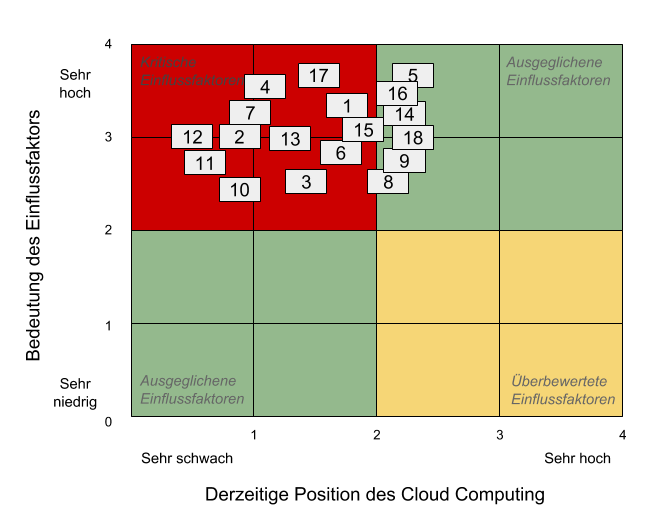
\includegraphics[width=\linewidth]{images/portfolio}
	\caption[Caption for parameters]{Faktorenportfolio}
	\label{fig:portfolio}
\end{figure}

\subsection{Einflussmatrix}

Die in Abbildung \ref{fig:matrix} dargestellte Einflussmatrix soll weiterhin wesentliche Treiber für den erfolgreichen Einsatz von Cloud Computing identifizieren. Eine Wertung von ''0'' kennzeichnet hier einen neutralen Einfluss eines Einflussfaktors auf einen anderen. Mit zunehmender Steigerung der Wertung steigt auch der Einfluss, d.h. eine ''3'' kennzeichnet einen starken Einfluss. 

Die Passivsummen geben eine Übersicht darüber, welche Faktoren stark von anderen beeinflusst werden. Die Faktoren mit einer hohen Passivsumme spielen keine große Rolle in der Gesamtwirkung und werden nachfolgend nicht weiter betrachtet.

Durch die ermittelte Aktivsumme lassen sich Einflussfaktoren erkennen, die im Folgenden näher betrachtet werden sollen. Hierzu werden alle Faktoren eingeschlossen, die eine Aktivsumme von gleich oder größer als 10 haben. Dazu gehören ''Informationssicherheit'', ''Störungssicherheit im Netzwerk'', ''Skalierbarkeit'', ''Zuverlässige und schnelle Datenübertragung'', ''Kontrollmöglichkeiten'', ''Orts - \& Zeitunabhängigkeit'' sowie ''Vernetzung von organisatorischen und prozessualen Strukturen''. Besonders das letztgenannte Kriterium fällt durch einen hohen Einfluss im Gesamtkontext hervor. Es lohnt sich somit, diesen Faktor gesondert zu betrachten. Die 7 ermittelten Faktoren mit der höchsten Aktivsumme werden nun als Schlüsselfaktoren identifiziert und nachfolgend genauer beschrieben.

\begin{figure}
	\centering
	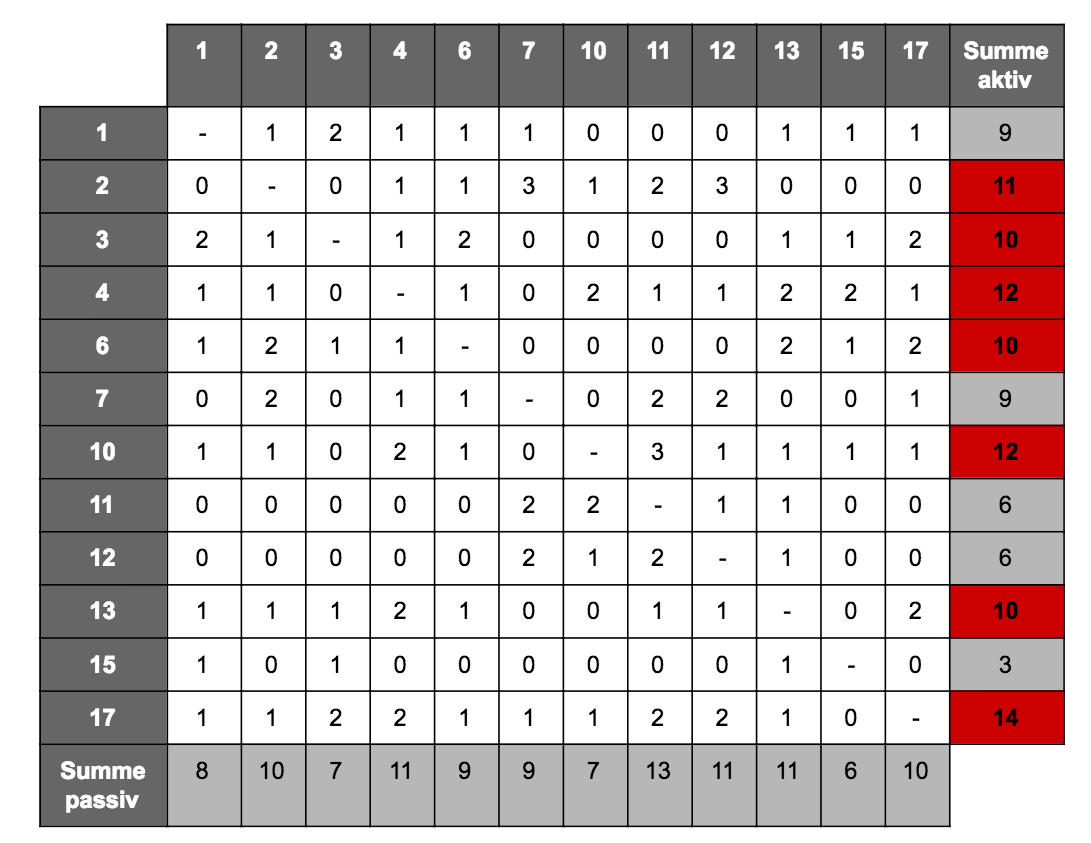
\includegraphics[width=\linewidth]{images/matrix}
	\caption[Caption for parameters]{Einflussmatrix}
	\label{fig:matrix}
\end{figure}

\subsection{Beschreibung der Schlüsselfaktoren}

Nachfolgend sollen die als Schlüsselfaktoren identifizierten Einflussfaktoren genauer beschrieben werden. Als erstes wurde \textit{Informationssicherheit} ermittelt. Innerhalb des Cloud Computing werden Daten zunehmend auf dezentrale Server gespeichert, die nicht mehr direkt im Unternehmen liegen, sondern in externen Rechenzentren \cite{krcmar}. Deshalb obliegt es einer enormen Wichtigkeit, diese Informationen gegen Systemangriffe zu schützen. Nur durch gewisse Sicherheitsvorkehrungen der angebotenen Cloud-Dienste kann ein generelles Vertrauen gegenüber der Technologie entstehen \cite{gebauer}.

Als zweiten Schlüsselfaktor wurde die \textit{Störungssicherheit im Netzwerk} genannt. Cloud Computing kennzeichnet ein hohen Grad an netzwerktechnischen System, gerade wenn ganze Infrastrukturen als Dienstleistung angeboten werden (vgl. IaaS) \cite{krcmar}. Diesbezüglich ist eine gewisse Stabilität des Netzwerkes enorm relevant. Gerade im Umfeld von Schulen, vor allem in ländlichen Regionen, ist eine stabile Netzwerkbandbreite eine generelle Anforderung \cite{gebauer}. Langsame Ladezeiten oder Nichtverfügbarkeit von Materialien durch störanfällige Netzwerke würden zu einer hohen Frustration führen.

Ein großes Schlagwort im Bereich des Cloud Computing ist die \textit{Skalierbarkeit} \cite{renz}. Angebotene Dienste müssen mit den Strukturen des Unternehmens oder mit den Anforderungen im digitalen Lernumfeld mitwachsen. Deshalb ist eine schnelle Anpassbarkeit der angebotenen Dienste auf Kundenwünsche generell sehr wichtig.

Im Kontext des zweiten Faktors (vgl. der Störungssicherheit) steht auch das Kriterium der \textit{zuverlässigen und schnellen Datenübertragung}. Gerade wenn es um die Übertragung von großen Datenmengen geht, ist die Leistungsfähigkeit der der angebotenen Dienste sehr relevant \cite{gebauer}.

Zwar hat der Benutzer durch die Verlagerung in die Cloud weniger Handhabung über seine Dienste, jedoch stehen die \textit{Kontrollmöglichkeiten} weiterhin im Vordergrund bei einer erfolgreichen Integration von Cloud Diensten. Hier ist es wichtig, dass der Kunde weiterhin durch flexible Bezahlungmodelle und dynamischen Skalierungsoptionen die Möglichkeit hat, die Dienste nach eigenen Bedürfnissen anzupassen. Dies ist vor allem wichtig im Bezug auf die Lokalisierung der Speicherorte der eigenen Orten, wenn gewisse Datenschutzbestimmungen erfüllt werden müssen \cite{gebauer}.

Gerade im Bezug des mobilen Lernens ist die \textit{Orts - und Zeitunabhängigkeit} ein sehr wichtiges Kriterium. Der Lernende soll jederzeit und an jedem Ort die Möglichkeit haben, auf Lernmaterialien zugreifen zu können \cite{grella}.

Abschließend stellt die \textit{Vernetzung von organisatorischen und prozessualen Strukturen} einer der wichtigsten Schlüsselfaktoren. Einer der großen Vorteile des Cloud Computing ist die Möglichkeit, viele Dienste über das Internet zu verbinden \cite{krcmar}. Dadurch können enorme Prozessoptimierungen vorgenommen werden, was für die Skola GmbH allein schon aus finanzieller Hinsicht ein wichtiges Indiz wäre.
  % Kapitel 4: Spezifikation von Einflussfaktoren
\section{Darstellung von Ausprägungen}
\label{manifestations}

Die zweite Phase der Szenarioanalyse bildet die Erstellung von Ausprägungen \cite{spath}. Hierfür werden Entwicklungspfade aus denen im vorhergehenden Kapitel definierten Schlüsselfaktoren gebildet. Im Folgenden wird somit für jeden Schlüsselfaktor eine sogenannte Trendprojektion bis hin zu einem bestimmten Punkt in der Zukunft erstellt \cite{mietzner}. Dieser wird grundsätzlich bis zu einer Spanne von 10 Jahren gesehen, da das Cloud Computing in seiner Entwicklung noch relativ am Anfang steht und eine zu weit entfernte Projektion sehr vage wäre. Als validierende Grundlage hierfür bildeten Experteninterviews sowie eine vertiefte Literaturrecherche.

\todo[inline]{todo} % Kapitel 5: Erstellen von Ausprägungen
\section{Szenariokonstruktion}
\label{constructions}
Als dritte und wichtigste Phase der Szenarioanalyse werden nun Szenarien aus den vorher definierten Einflussfaktoren erstellt. Hierfür bietet es sich an, die vorher ermittelten Entwicklunsausprägungen der einzelnen Schlüsselfaktoren auf Widerspruchsfreiheit zu überprüfen . Dafür wird eine Konsistenzanalyse genutzt \cite{spath}. Auf dessen Grundlage werden danach zukunftsfähige Anwendungsszenarien für die Skola GmbH erstellt.

\subsection{Konsistenzanalyse}

In der in Abbildung \ref{fig:konsistenzanalyse} dargestellten Konsistenzanalyse erhält man eine Übersicht über die Beziehung zwischen den einzelnen Ausprägungen. Der Übersichtlichkeit halber wurden die einzelnen Ausprägungen abgekürzt. Die Erklärungen finden sich in Abschnitt \ref{manifestations}.

\begin{figure}
	\centering
	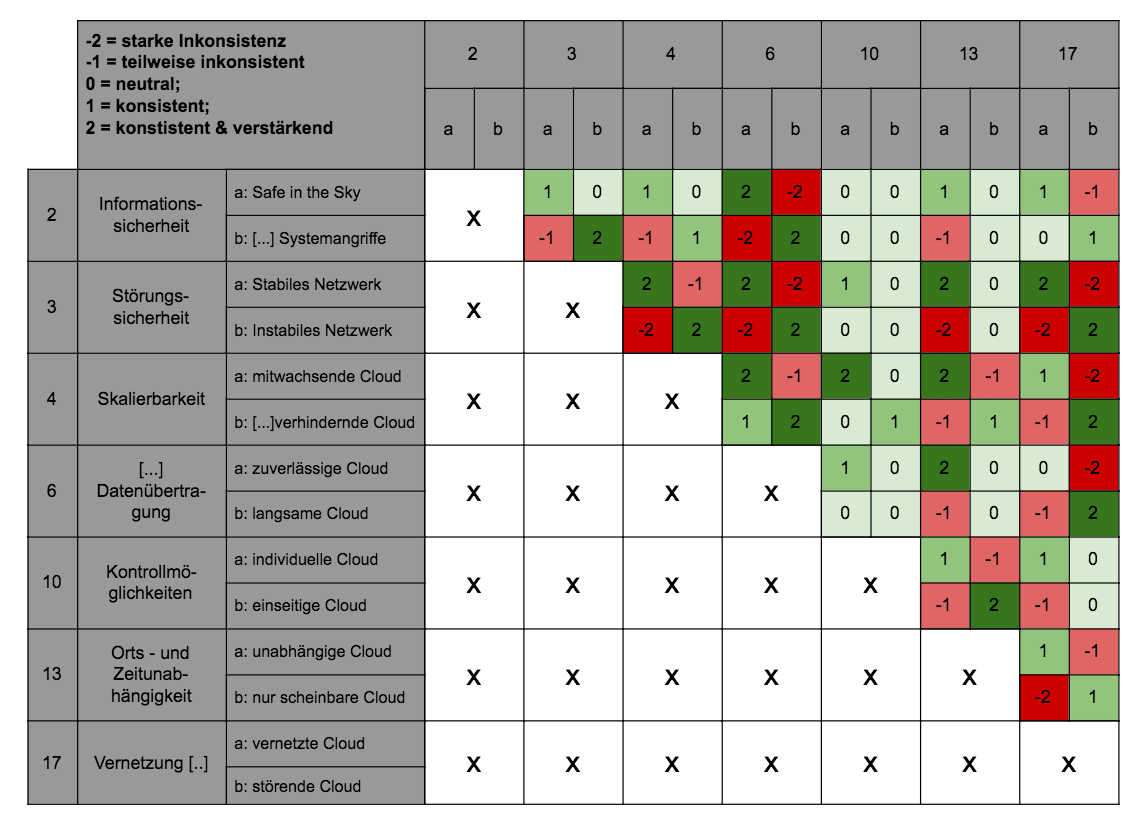
\includegraphics[width=\linewidth]{images/konsistenzanalyse}
	\caption[Caption for parameters]{Konsistenzanalyse}
	\label{fig:konsistenzanalyse}
\end{figure}

Für die Konsistenzanalyse wurde eine Skala zwischen -2 (starke Inkonsistenz) und 2 (konsistent und verstärkend) gewählt. Faktorenausprägungen, die eine starke Inkonsistenz aufweisen, können nicht zusammen in einem Szenario aufgeboten werden \cite{spath}. Andersrum können aus verstärkenden Ausprägungen Cluster gebildet werden, woraus sich Szenarien abbilden lassen.

Aus der Analyse der Schlüsselfaktoren auf Widerspruchsfreiheit lässt sich sehr gut erkennen, dass sich die jeweiligen Best-Case Ausprägungen zumeist verstärken. Besonders lässt sich ein positives Cluster aus den Ausprägungen \textit{Stabiles Netzwerk} (3a), \textit{mitwachsende Cloud} (4a), \textit{zuverlässige Cloud} (6a) und \textit{unabhängige Cloud} zusammenfassen. Andere positive Ausprägungen lassen sich zudem hinzuaddieren, sodass sie weiterhin verstärkend wirken. Im Gegensatz dazu verstärken sich die negativen Ausprägungen der Schlüsselfaktoren, wodurch sich ein entsprechendes negatives Cluster bilden lässt.

Aus dieser Betrachtung lässt sich erschließen, dass sich die Vorteile des Cloud Computing generell verstärkend aufeinander auswirken. Ebenso unterstützen sich die Risiken gegenseitig in ihrer Ausprägung. Diese Erkenntnis kann nun zur Hilfe gezogen zu werden, um drei mögliche Zukunftsszenarien für das Cloud Computing im Bildungsbreich zu erstellen.

\subsection{Szenario 1 - Mobiles Lernen auf dem Vormarsch}

In diesem Zukunftsszenario haben die positiven Ausprägungen des Cloud Computing Einklang in den Lernalltag von Schülerinnen und Schülern gefunden. Mobiles Lernen ist kein Ideal mehr sondern ein allgemeiner Zustand. Lernende haben jederzeit und überall Zugang zu Materialien über das Internet. E-Learning gehört ebenso zum Alltag wie eigenverantwortliches Nacharbeiten zu Hause mit dem eigenen Smartphone oder Tablet. Den Schülerinnen und Schülern wird Platz für freie Entfaltung gegeben, klassischer Unterricht besteht nur noch geringfügig. Schulbücher in der Form wie man sie aus klassischen Lernprinzipien kennt existieren bestenfalls als Zusatzmaterial. Große Schulbuchverlage wie Cornelsen oder Westermann haben ihre Angebote längst ins Internet mithilfe von Cloud Services verlagert. Dadurch bieten sie flexible, aber auch zahlreiche Lernmaterialien für jeden an. Zudem sind die angebotenen Dienstleistungen jederzeit sicher und entsprechen sämtlichen Datenschutzrichtlinien. 

In Betrachtung der derzeitigen Entwicklung des Cloud Computing ist ein solches Szenario in den nächsten 10-15 Jahren denkbar. Der Gebrauch der Technologie wächst immer weiter an \cite{krcmar} und Firmen der deutschen Bildungsindustrie überdenken ihr Angebot hinsichtlich eines Wechsels zu cloudbasierten Diensten \cite{grella}.

\subsection{Szenario 2 - Blended Learning (Hybrid)}

Dieses Szenario sieht ein Mischmodell aus Online - und Offline-Angebot von Unterrichtsmaterialien vor. Dies entspricht der in Abschnitt \ref{futuretrends} vorgegebenen Definition des \textit{Blended Learning}. Es sollen Synergien beider Modelle genutzt werden, um Vorteile beider Seiten auszunutzen und Nachteile möglichst zu beseitigen. Das Szenario sieht vor, dass Schülerinnen und Schüler eigenständig Hausaufgaben oder Nachholarbeiten über das cloudbasierte Web Services vornehmen, zum Beispiel durch E-Learning Angebote. Weiterhin bestehend bleibt aber der eigentliche Präsenzunterricht. Unterstützt wird dieser durch passende Web Services, die den Unterricht didaktisch bereichern \cite{meinel}.

Dieses Szenario ist ebenfalls in den nächsten 10-15 Jahren als ziemlich realistisch einzuschätzen. Zwar bleibt das Vertrauen in bewehrte Unterrichtskonzepte, auch hervorgerufen durch die Angst vor Datenschutzverletzungen, jedoch steigt der Einsatz von Cloud Diensten rasant \cite{krcmar}. 

\subsection{Szenario 3 - Zu hohe Risiken}

Eher unwahrscheinlich ist das dritte Szenario, welches beschreibt, dass Cloud Computing gar keinen Einklang in die Bildungsbranche finden wird. In diesem Fall sind die abgeschätzten Risiken der Technologie zu groß, um ernsthaft Vertrauen in eine Verlagerung von Lernmaterialien in die Cloud zu gewinnen. Hier wird weiter bewährte, klassische Konzepte vertraut. 

Unrealistisch ist dies deshalb, weil die Vorteile des Cloud Computing bei weitem überwiegen. Zwar gibt es berechtigte Risiken, wie zum Beispiel die Datensicherheit oder die Störanfälligkeit der bereitgestellten Infrastrukturen, diese können jedoch durch geeignete Konzepte eingeschränkt werden.

 % Kapitel 6: Szenariokonstruktion
\section{Zusammenfassung und Handlungsempfehlungen}
\label{conclusion}
Aus den erarbeiten Zukunftsszenarien ergeben sich nun Handlungsempfehlungen für die fiktive Skola GmbH. Diese können dementsprechend auf die tatsächliche Situation in der Bildungsbranche angewendet werden.

Die in Abschnitt \ref{constructions} gezeigten Szenarien haben gezeigt, dass ein Einsatz von Cloud Services durch das Unternehmen durchaus sinnvoll ist (vgl. Szenario 1 und 2). Dies kann auf unterschiedlichem Wege passieren. Als Schulbuchhersteller kann die Skola GmbH auf bereits vorhandene Ressourcen in Form ihrer Schulbücher sowie Arbeitsmaterialien zurückgreifen und diese beispielsweise als eigenständiger Cloud Provider im Internet anbieten. Dadurch kann man auf die Zukunftstrends \textit{mobiles Lernen}, \textit{E-Learning} oder \textit{Blended Learning} aufspringen. Man kann hierbei in alternative Richtungen gehen. Zum Beispiel könnte man im Bezahlmodell oder in der Art der angebotenen Dienste variieren (vgl. Abschnitt \ref{environment}). Dazu ist zwingend technisches Know-How notwendig. 

Will man als eigenständiger Provider auftreten, muss man zudem die Risiken der Cloud Technologie berücksichtigen (vgl. Szenario 3). Eine Reduzierung der Probleme kann zum Beispiel durch eine Verlagerung dieser Dienste auf externe Cloud Provider vorgenommen werden, wie zum Beispiel \textit{Amazon Web Services} oder \textit{Google Cloud Platform}. Dadurch liegt ein Großteil der Verantwortung bei den externen Anbietern und man kann sich auf die Bereitstellung der Lernmaterialien konzentrieren.

Wichtig in diesem Kontext ist zudem die Problematik des Datenschutzes. Geht man zum Beispiel den Weg über externe Dienstleister, muss beachtet werden, dass diese gegenwärtigen Richtlinien entsprechen. Gerade bei ausländischen Anbietern ist dies momentan schwer oder gar nicht gewährleistet. Kritisch in diesem Zusammenhang ist zudem der vorhandene Bildungsförderalismus in der deutschen Lernindustrie.

Grundsätzlich lässt sich jedoch zusammenfassen, dass das Cloud Computing enorme Potentiale im Bildungsbereich bietet. Es ist zunehmend wichtig, die Vorteile der Technologie zu bündeln, um diese Potentiale ausschöpfen zu können. Essentiell ist hierbei ein bundesweit einseitiges, datenschutzrechtliches ansprechendes Konzept. % Kapitel 7: Zusammenfassung und Handlungsempfehlungen

\begin{thebibliography}{00}
\bibitem{bitkom}M. Vogel und A. Pols, ''Cloud Monitor 2017“, Berlin, 2017
\bibitem{meinel2} C. Meinel, J. Renz, C. Grella, N. Karn, und C. Hagedorn, ''Die Cloud für Schulen in Deutschland: Konzept und Pilotierung der Schul-Cloud", Potsdam, 2017.
\bibitem{spath}D. Spath, S. Schmipf, und C. Lang-Koetz, ''Technologiemonitoring - Technologien identifizieren, beobachten und bewerten“, Stuttgart, 2010.
\bibitem{grella} C. Grella, N. Karn, J. Renz, und C. Meinel, ''Schulrechner wandern in die Cloud – Was bedeutet das für die unterschiedlichen Stakeholder?“, Bonn, 2017.
\bibitem{specht} M. Specht, M. Kalz, und D. Börner, ''Innovation und Trends für mobiles Lernen“, Wiesbaden, 2013.
\bibitem{stieninger} M. Stieninger, ''Der Einsatz von Cloud Computing in KMU – Einflussfaktoren für Diffusion und Akzeptanz“, Steyr, 2013.
\bibitem{krcmar} H. Krcmar, J. M. Leimeister, A. Roßnagel, und A. Sunyaev, Hrsg., ''Cloud-Services aus der Geschäftsperspektive", Wiesbaden, 2016.
\bibitem{mietzner} D. Mietzner, ''Strategische Vorausschau und Szenarioanalysen", Wiesbaden, 2009.
\bibitem{zpunkt}zpunkt gmbh, „zPunkt Megatrends update“, Köln, 2018.
\bibitem{goertz} L. Goertz, ''Digitales Lernen adaptiv - Technische und didaktische Potenziale für die Weiterbildung der Zukunft“, Gütersloh, 2014.
\bibitem{gebauer} L. Gebauer, M. M. Gierczak, M. Söllner, und J. M. Leimeister, ''Einflussfaktoren auf die Nutzung von Cloud-Speicherdiensten“, Wiesbaden, 2015.
\bibitem{schweizer} M. Schweizer, ''Studie cloud migration 2018“, München, 2018.
\bibitem{meinel} C. Meinel, ''Die Mitglieder der Arbeitsgruppe 1 ‚Digitale Bildungsplattformen: Innovationen im Bildungsbereich‘“, Saarbrücken, 2016.
\bibitem{almajalid} R. Almajalid, ''A Survey on the Adoption of Cloud Computing in Education Sector“, Jeddah, 2017.
\bibitem{chandra} D. G. Chandra und D. Borah Malaya, ''Role of cloud computing in education“, New Delhi, 2012.
\bibitem{renz} N. Kiefer, ''Experteninterview mit Jan Renz zum Thema Cloud Computing in der Bildungsbranche", Wernigerode, 2018.
\bibitem{alabbadi} M. M. Alabbadi, ''Cloud computing for education and learning: Education and learning as a service (ELaaS)“, Riyadh, 2011.
\bibitem{stute} P. Stute, ''Interview mit Philipp Stute zum Thema Cloud Computing: Chancen, Risiken und Nebenwirkungen“, Augsburg, 2013.
\bibitem{velten} C. Velten, ''Cloud Computing – Backbone der Digitalisierung“, Kassel, 2018.
\bibitem{karlstetter} F. Karlstetter, ''Rückblick und Ausblick auf den Cloud-Markt“. [Online]. Verfügbar unter: https://www.cloudcomputing-insider.de/rueckblick-und-ausblick-auf-den-cloud-markt-a-675571/. [Zugegriffen: 10-Mai-2018].

\end{thebibliography}

\end{document}
